\chapter{Experiment And Results}
\minitoc

\section{Dataset}

The dataset used in this experiment is called AliCPP and it is a public dataset that contains user-item interactions from an e-commerce platform. The dataset gather traffic logs of recommendation systems in Taobao, a Chinese online shopping website. The dataset is collected from the real-world recommendation system of Taobao.\cite{AliCPP}


\section{Experimental Setup}

In order to evaluate the performance of the proposed solution with real-world data, the environment has to be accelerated with a GPU.

\subsection{Hardware Environment}

To achieve this, the experiment is conducted on a cloud-based environment, specifically on an AWS EC2 p3.2xlarge instance \cite{AwsEc2P3}.

The instance is equipped with 8 vCPUs, 61 GiB of memory, and a single NVIDIA Tesla V100 GPU.

The V100 is a high-end GPU that is designed for AI workloads especially deep learning tasks.
It is based on the Volta architecture and is equipped with 5120 CUDA cores, 640 Tensor cores, and 32GB of HBM2 memory with 1.1 TB/s.
It can deliver 7 TFLOPS of double-precision floating-point performance and 116 TFLOPS of deep learning performance.

Figure \ref{fig:V100vsCPU} shows the performance comparison between the Tesla V100 and a CPU.


\begin{figure}[H]
    \centering
    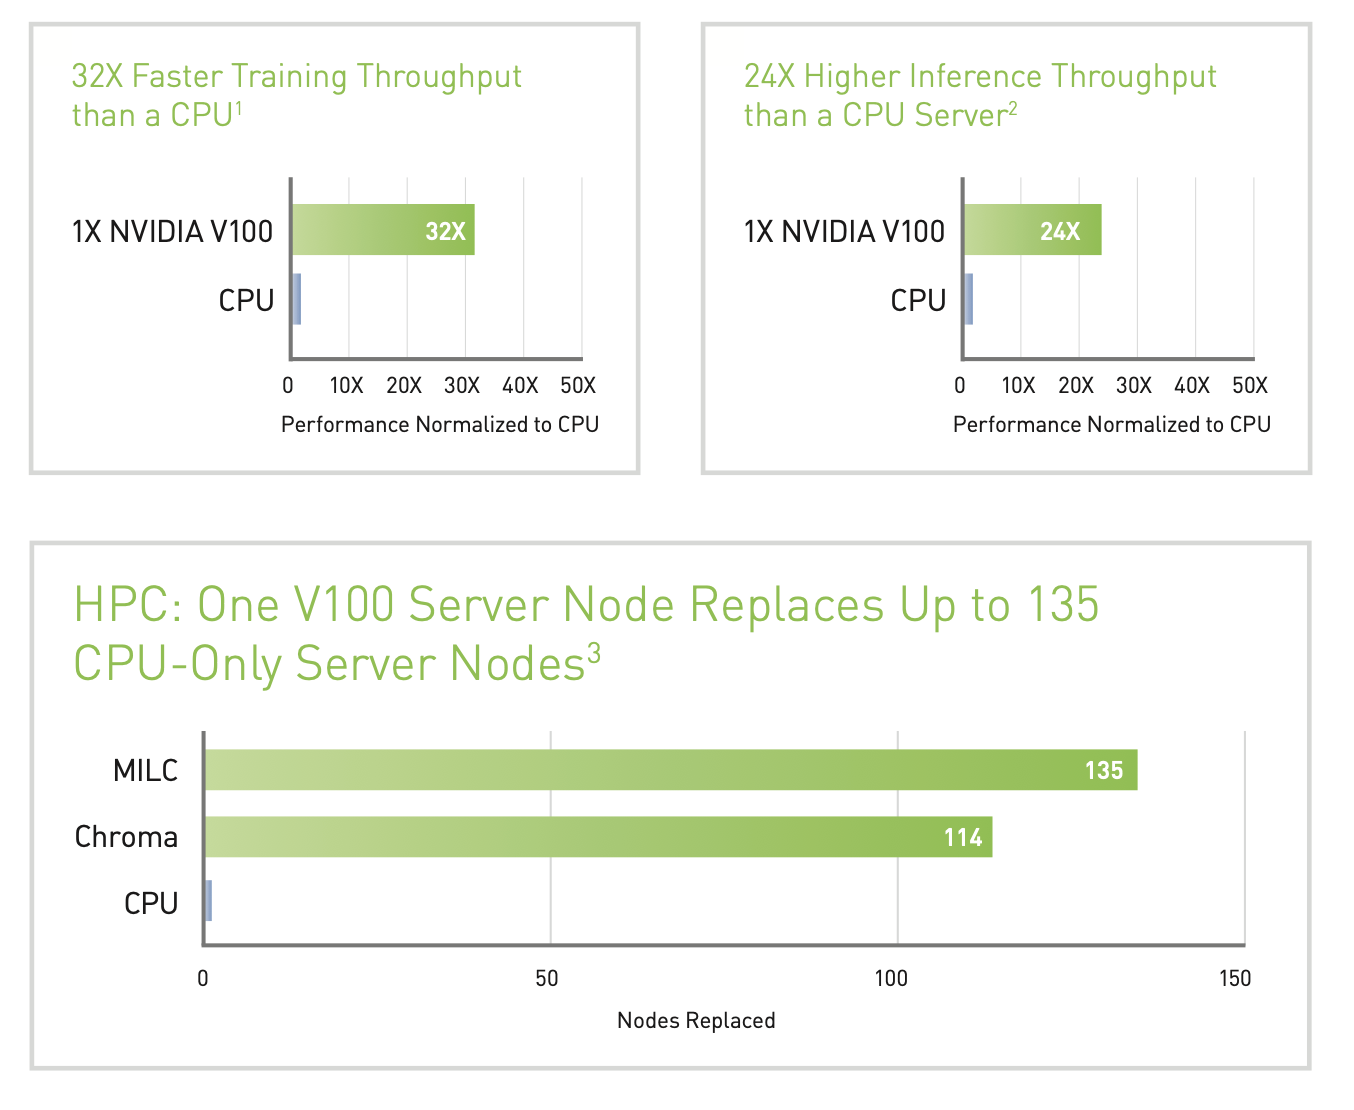
\includegraphics[width=0.8\textwidth]{assets/v100-vs-cpu.png}
    \caption[Tesla V100 vs CPU]{Tesla V100 vs CPU \cite{NvidiaV100DataSheet}}
    \label{fig:V100vsCPU}
\end{figure}

\subsection{Software Environment}

In addition to the hardware environment, the software environment is also important to be considered.
Having access to \textbf{Nvidia Inception Program} \cite{NvidiaStartups}, 
which includes access to NVIDIA AI Enterprise \cite{NvidiaAiEnterprise} with \textbf{Nvidia GPU Cloud (NGC) Catalog}\cite{NvidiaNGC}.

Instead of setting up the drivers, tools, libraries and frameworks manually, 
the Nvidia AI Enterprise provides a pre-configured flavor of Linux Ubuntu that includes all necessities for deep learning tasks.

In addition to that, instead of compiling the Merlin TensorFlow from the source code, 
the Nvidia Merlin TensorFlow Container \cite{NvidiaMerlinTf} was used as a runtime for the experiment Jupyter notebook.



\section{Evaluation Metrics}